\documentclass[11pt, conference]{article}
\usepackage[left=4cm, right=4cm, top=3cm, bottom=3cm]{geometry}
\usepackage{graphicx}
\usepackage{cite}
\usepackage{algorithmic}
\usepackage{graphicx}
\usepackage{textcomp}
\usepackage{balance}
\usepackage{comment}
\usepackage{grffile}
\usepackage{subcaption}
\usepackage{lipsum}
\usepackage{float}

\newcommand{\vectorScheme}{\textit{Vector Scheme}}
\newcommand{\valueScheme}{\textit{Value Scheme}}
\newcommand{\distanceScheme}{\textit{Distance Scheme}}
\newcommand{\distanceLemma}{\textit{Distance Lemma}}
\newcommand{\sketchScheme}{\textit{Sketched Data Scheme}}
\newcommand{\fullSync}{\textit{Full Sync}}
\newcommand{\naiveScheme}{\textit{Naive Scheme}}
\newcommand{\oracleScheme}{\textit{Oracle Scheme}}
\newcommand{\falseAlarm}{\textit{false alarm}}
\newcommand{\falseAlarms}{\textit{false alarms}}
\newcommand{\coveringSpheres}{\textit{Covering Spheres}}
\newcommand{\convexDecomposition}{\textit{Convex Decomposition}}
\newcommand{\convexBound}{\textit{Convex Bound}}
\newcommand{\theCoordinator}{\textit{the coordinator}}
\newcommand{\Coordinator}{\textit{Coordinator}}
\newcommand{\TheCoordinator}{\textit{The coordinator}}
\newcommand{\safeZone}{\textit{safe zone}}

\begin{document}
	\begin{titlepage}
		\begin{center}
			\vspace*{1cm}
			\begin{Huge}
				Thesis Proposal \\
			\end{Huge}
			\vspace{1cm}
			\line(1,0){300} \\
			\vspace{0.2cm}
			\begin{Huge}
				Bandwidth Efficient Distributed Monitoring Schemes \\
			\end{Huge}
			\line(1,0){300} \\
			\vspace{1.5cm}
			\begin{Large}
				Yuval Alfassi \\
			\vspace{1cm}
				Supervised by Prof. Daniel Keren \\
			\vspace{2.5cm}
				University of Haifa \\
				Faculty of Social Sciences \\
				Department of Computer Science \\
			\vspace{1.5cm}
				December, 2018 \\
			\end{Large}
		\end{center}
	\end{titlepage}

\newgeometry{top=1.5in,bottom=1.5in,right=1in,left=1in}

\section*{Abstract}

Distributed monitoring is a problem that arises when trying to monitor properties of dynamic data which is spread distributively. Tracking the value of a function over dynamic data in a distributed setting is a challenging problem in numerous real-world modern applications. Several monitoring schemes were proposed as an approach to coping with this problem in order to reduce the amount of communication messages between servers.

This research will focus on developing new distributed monitoring schemes which use much less communication bandwidth than existing methods. This will be done by exploiting some unique properties of convex functions so that the dimensionality of the transmitted data will be reduced.

\section{Introduction}

Monitoring a function over a large amount of dynamically changing data in a distributed fashion is a common computer-science challenge. Whether it's monitoring features of distributed sensor networks \cite{burdakis2012detecting}, top-k monitoring \cite{babcock2003distributed}, monitoring distributed ratio queries \cite{gupta2013ratio} or tracking properties of large distributed dynamic graphs \cite{mcgregor2015densest}, innovative approaches had to be developed in order to deal with the difficulties of the data being both dynamic and distributed.

The need for minimizing both the bandwidth and the processing power is described in \cite{giatrakos2013network}; in the \textit{Big Data} era, where data is of very high dimensionality and changes rapidly, data transmission over a communication channel has to be devised cleverly. Transmition of high dimensional data is not only extremely time consuming but also virtually impractical; for instance, a system of air pollution sensors which distributively have to determine the air pollution level may benefit from communication reduction \cite{cheng2004revised}.

\subsection{Problem Definition}

Commonly, the distributed monitoring model is focused on determining whether a function over dynamic distributed data crosses a certain threshold. This is used as a component to the \textit{distributed function approximation problem} \cite{garofalakis2013sketch}, which $\varepsilon$-approximates the value of a function over time. The distributed model is described as follows:
\begin{enumerate}
\item There are $n$ data-servers, $s_1 ... s_n$
\item A central \textit{coordinator} $c$ exists, with whom the servers communicate over a communication channel.
\item Server $s_i$ knows only its dynamic data -- the local vector, $v_i$.
\item The global data, represented by the global vector $v$, is the average of the local vectors:
\begin{equation}
v = \frac{1}{n}\sum\limits_{i=1}^n {v_i}
\end{equation}
\item A function $f$ is monitored over the global vector $v$ so it's $\varepsilon$-approximated with 100\% confidence: let the estimation be the dynamic value $\mu$ (without loss of generality, assume ${\mu \geq 0}$), then at all times: 
\begin{equation}
(1-\varepsilon )\mu \leq f(v) \leq (1+\varepsilon )\mu
\end{equation}
\end{enumerate}

The \textit{threshold monitoring problem} \cite{garofalakis2013sketch}  monitors whether the function's value crosses a certain threshold. The function approximation problem is commonly reduced to two simultaneous threshold monitoring problems: let ${T = (1+\varepsilon )\mu}$ be the upper-bound threshold's value, then, the upper-bound monitoring objective is to determine whether:
\begin{equation}
f(v) \leq T
\end{equation}

Likewise, the lower-bound function monitoring is performed with the threshold ${(1-\varepsilon )\mu}$.

In turn, this threshold monitoring can be treated as a \textit{geometric monitoring problem} \cite{sharfman2007geometric}, where one tries to find a \safeZone \ of vectors ${\{v \ | \ f(v) \leq T\}}$, which is convex, so every convex combination of vectors inside this safe zone is also inside the safe zone, see Fig. \ref{fig:ConvexSafeZoneSketch}. This geometric safe zone approach is the fundamental idea behind distributed monitoring techniques.

\begin{figure}[h]
\begin{center}
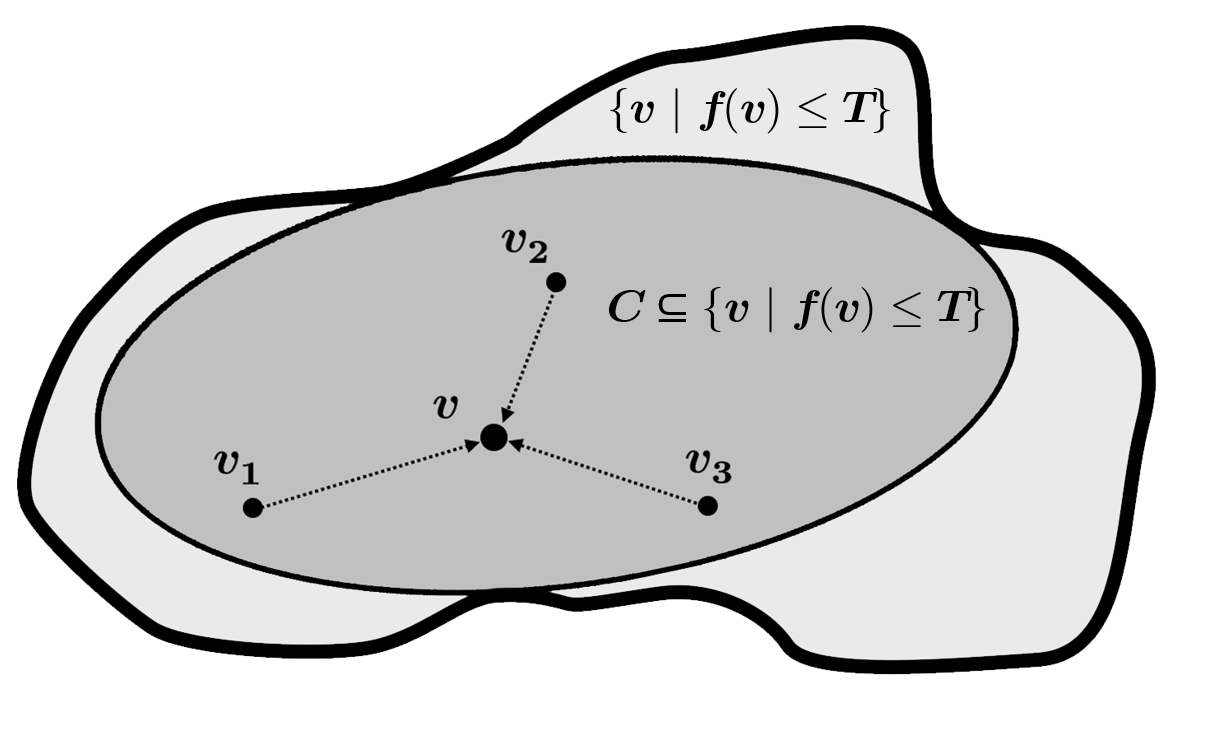
\includegraphics[width=0.7\linewidth]{Pics/PNGs/ConvexSafeZone.png}
\end{center}
\caption{Convex Safe Zone}
\label{fig:ConvexSafeZoneSketch}
\medskip
\small
\begin{center}
$C$ is a convex bound of the set ${\{v \ | \ f(v) \leq T\}}$; since ${v_1,v_2,v_3 \in C}$, so does the average vector $v \in C$.
\end{center}
\end{figure}

\section{Previous Work}

\subsection{Linear Functions}

Since linear functions are additive and homogeneous, the basic algorithm for distributively monitoring their value is fairly easy. Since ${f(v) = \frac{1}{n}\sum f(v_i)}$, tracking the value of the global $f(v)$ isn't quite complicated. Work about linear functions such as the distributed count problem was done at \cite{keralapura2006communication}. However, things get more complicated when dealing with non-linear functions.

\subsection{The Covering Spheres Method}

The first approach which exploited the geometric view of the ditributed monitoring problem is the \coveringSpheres \ method \cite{sharfman2007geometric}.

This method artificially creates a convex safe zone (as shown in Fig. \ref{fig:ConvexSafeZoneSketch}) where the server's local data could be at without a need for communication.

This method seemed very effective theoratically, though it proved to be impractical. The \coveringSpheres \ method demands performing lots of time consuming heavy mathematical operations, so it isn't scalable computation-wise \cite{lazerson2018lightweight}.

Furthermore, the violation resolution phase demands transmitting high dimensional vectors, which makes the communication bandwidth quite too high.

\subsection{The Convex Decomposition Method}

Another distributed monitoring scheme previously developed is the \convexDecomposition \ method \cite{lazerson2015monitoring}. This method composes a convex safe zone by decomposing into half-planes the geometric space of the monitored condition. The \convexDecomposition \ method geometrically monitors whether the average global vector is in the intersection of the half-planes.

Unfortunately, this method suffers from similar issues as the \coveringSpheres \ method, and cannot be applied on some basic functions, thus isn't always feasable \cite{lazerson2018lightweight}

\subsection{The Convex Bound Method}

The \coveringSpheres \ method and the \convexDecomposition \ method turned out to be impractical albeit their mathematical foundation. In need of more computationally lightweight and consistent monitoring approach, the \convexBound \ method was proposed \cite{lazerson2018lightweight}.

The \convexBound \ method tightly bounds the monitored function by a convex function, so the convex bound serves as the convex safe zone: when monitoring $f(v) \leq T$, an upper bound convex $c$ has to be found so for all $v$, $f(v) \leq  c(v)$.

And the new monitoring objective becomes:
\begin{equation}
\label{monitoringConstraint}
c(v) \leq T
\end{equation}

The same goes for lower bound threshold monitoring -- it's done by bounding $f$ from below by a concave function.

Accordingly, the distributed function monitoring is performed on the convex bound functions, which is far simpler due to the convexity property. On the other hand, this method is also very expensive regarding the bandwidth consumption; high dimensional data is frequently transmitted on the communication channel.

\section{Research Objectives}

The research will focus on developing innovative distributed monitoring schemes which will reduce the communication bandwidth of the distributed monitoring process. Specifically, we'll try:

\begin{enumerate}
\item Incorporating data-sketches into the \convexBound \ method without damaging the 0\% false-negative necessity of the distributed monitoring problem.

\item Proving the \distanceLemma , a lemma used as a basis of an efficient distributed monitoring scheme we'll develop. The \distanceLemma \ states that given a convex body and several points, if the sum of distances to the convex border from the points inside the convex body is greater than the sum of distances to the border from the points outside, then the average of the points is inside the convex body. Thus, distributed monitoring can be performed by sending just one scalar -- the distance to the convex body.

\item Conducting several experiments, laying out comparisons of multiple attributes of distributed monitoring schemes on real-world data, focusing on the bandwidth consumption.
\end{enumerate}

\bibliographystyle{ieeetran}
\bibliography{References}
	
\end{document}